\subsection{Misura della Corrente Massima}

\begin{wrapfigure}[14]{l}{0.55\textwidth}
  \begin{center}
    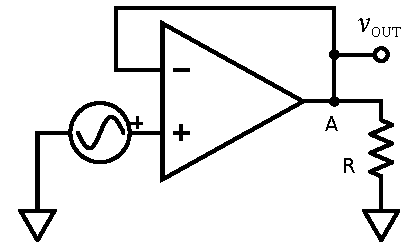
\includegraphics[width=0.26\textwidth]{../E03/latex/max_current.pdf}
  \end{center}
  \caption{Schema del circuito utilizzato per misurare la corrente massima. La resistenza utilizzata è $R=98.47\pm0.01$\si{\ohm}.}
  \label{cir2:max_current}
\end{wrapfigure}

L'amplificatore operazionale ha una corrente massima di uscita che può gestire; ai capi di un carico a bassa impedenza non riesce quindi ad erogare abbastanza corrente per amplificare il segnale, creando un clip. Per misurare tale corrente abbiamo dunque sfruttato questo fatto, ponendo una resistenza di carico fra l'uscita dell'operazionale e terra \footnote{Si noti che, data l'alta impedenza in ingresso dell'oscilloscopio ($1$ \si{\mega\ohm}), non era possibile misurare la corrente massima con questo strumento (attesa, come da specifiche del costruttore, sui $15$ \si{\milli\ampere}): sarebbe servita una tensione di $15000$ \si{\volt}!}, con l'oscilloscopio ai capi di tale resistenza per la misura di tensione (circuito in Figura ???????).

Sfruttando la legge di Ohm otteniamo, misurando la tensione a cui avviene il clip (con la funzione cursore dell'oscilloscopio), il valore di corrente massimo erogabile dall'OPAMP risulta

$$I_{max} = \frac{V_{clip}}{R}$$

Bisogna però considerare che la corrente, ponendo il segnale in entrata in alternata, risulta oscillare fra valori negativi e positivi (corrente rispettivamente entrante o uscente dal punto A). Inoltre, tali valori sono differenti (si nota dal grafico in Figura ?????? l'asimmetria della tensione di clip):

$$I_{V^+} = \frac{0.9625 \si{\volt}}{R} = 9.8 \si{\milli\volt}  \qquad I_{V^-} = \frac{1.7250 \si{\volt}}{R} = 17.5 \si{\milli\volt}$$